%{{{ Präämbel
\documentclass{beamer} %% normal document
%\documentclass[notes]{beamer} %% notes in normal document
%\documentclass[draft,notes]{beamer} %% draft with notes
%\documentclass[handout]{beamer} %% handout

\usepackage{fontspec, unicode-math, caption}
\usepackage[ngerman]{babel}
\usepackage{graphicx}
\usepackage{float}
\usepackage{enumitem}

%% usefull for handout with blank lines
%\usepackage{handoutWithNotes}
%\pgfpagesuselayout{2 on 1 with notes}[a4paper,border shrink=5mm]

%% usefull for presentation
%\setbeameroption{show notes on secondscreen=left}

\definecolor{bettergreen}{rgb}{.1,.7,.1}

\usetheme{Dresden}
\usecolortheme[named=bettergreen]{structure}
\useoutertheme{split}
\setbeamertemplate{caption}[numbered]
\captionsetup{labelformat=simple,font=scriptsize,labelfont=scriptsize}

% puts Frame numbers in Dresden template
\newcommand*\oldmacro{}%
\let\oldmacro\insertshorttitle%
\renewcommand*\insertshorttitle{%
	\oldmacro\hfill%
	\insertframenumber\,/\,\inserttotalframenumber}

\title[]{}

%{{{
\author{
	Johannes Visintini, Philip Bell,\\
	Moritz Nöltner, Andrii Soliar
}
%}}}


%{{{
\institute[IFI]{
	Vorlesung: Einführung in Software Engineering\\
	Institut für Informatik\\
	Universität Heidelberg
}
%}}}

%}}}

%{{{
\begin{document}

	%{{{
	\begin{frame}[plain]
		\titlepage
		\note{ }
	\end{frame}
	%}}}

	%{{{
	%%\section*{Teampräsentation}
	\begin{frame}{Teampräsentation}
		\center{\huge Die ASDF-Group}
		\vspace{2em}
		\begin{itemize}
			\item Philip Bell\\
				B.Sc. Mathematik, 5. Fachsemester
			\item Moritz Nöltner\\
				B.Sc. Angewandte Informatik, 5. Fachsemester
			\item Andrii Soliar\\
				B.Sc. Angewandte Informatik, 4. Fachsemester
			\item Johannes Visintini\\
				B.Sc. Angewandte Informatik, 5. Fachsemester
		\end{itemize}
	\end{frame}
	%}}}

	%{{{
	\section{Bisheriger Zustand}
	\begin{frame}{Bisheriger Zustand}
		\begin{figure}[H] %% There is no sense in having this image appear somewhere else
			\centering
			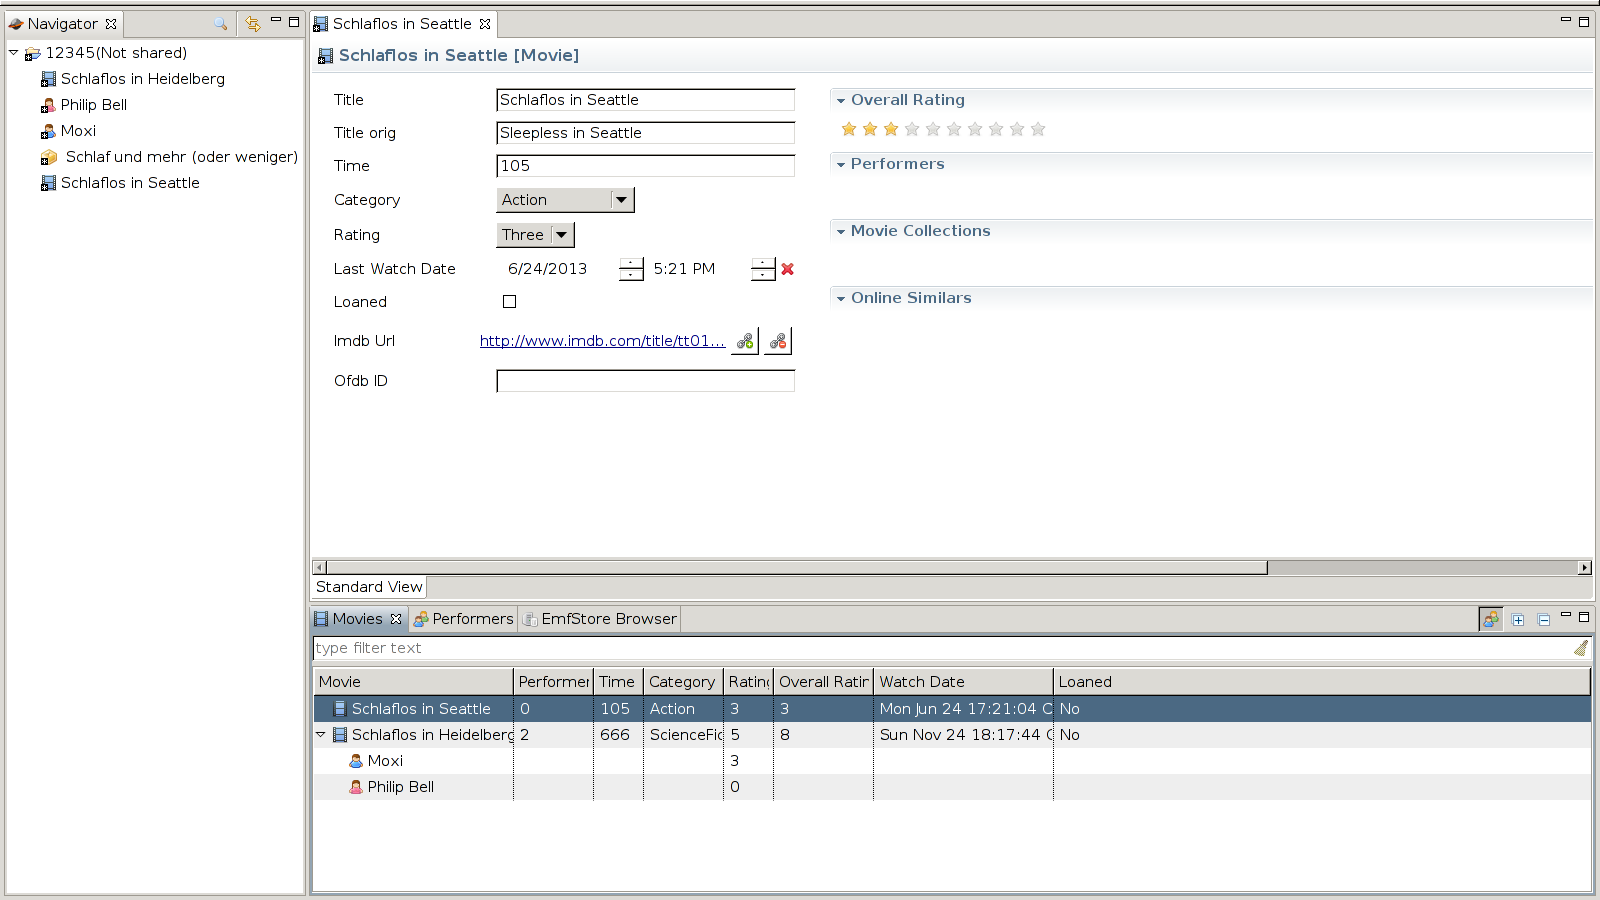
\includegraphics[width=\linewidth]{moviemanager_all}
			%\caption{Tuchulcha with a (very) simple workflow, picture taken from \cite{tuchulcha-website}}
		\end{figure}
	\end{frame}
	%}}}

	%{{{
	\section{Verbesserungsvorschläge}
	\subsection{Probleme und Lösungen}
	\begin{frame}{Probleme und Lösungen}
		\begin{columns}[c]
			\begin{column}{0.5\textwidth}
				\begin{itemize}
					\item 
\includegraphics[height=\baselineskip]{material/dialog-cancel.png} Viel manuelle Eingaben nötig
					\item 
\includegraphics[height=\baselineskip]{material/dialog-cancel.png} Angaben möglicherweise unvollständig
					\item 
\includegraphics[height=\baselineskip]{material/dialog-cancel.png} Angaben möglicherweise unkorrekt
				\end{itemize}
			\end{column}
			\pause
			\begin{column}{0.5\textwidth}
				\begin{itemize}
					\item 
\includegraphics[height=\baselineskip]{material/dialog-ok.png} Manuelle Eingabe minimiert
						\pause
					\item 
\includegraphics[height=\baselineskip]{material/dialog-ok.png} Eingabe autovervollständigt
						\pause
					\item 
\includegraphics[height=\baselineskip]{material/dialog-ok.png} unkorrekte Eingaben hervorgehoben
				\end{itemize}
			\end{column}
		\end{columns}
	\end{frame}
	%}}}

	%{{{
	\subsection{Umsetzung}
	\begin{frame}{Umsetzung}
		\small
		\begin{tabular}{p{1.7cm} p{2.6cm} p{2.6cm} p{2.3cm} }
			\textbf{Funktion} & \textbf{Beschreibung} & \textbf{Eingabe} & \textbf{Ausgabe} \pause \\
			\\
			Complete & vervollständigt mit IMDB & Titelanfang, orig. Title, Time, Category, IMDB-Url & Array of {Title, IMDB-Url} \pause \\
			\\
			Validate & prüft eingegebene Werte & Title, orig.~Title, Category, IMDB-Url, do~not~validate? & rote~Fläche, grüne~Fläche \\
		\end{tabular}
	\end{frame}
	%}}}

	%{{{
	\subsection{Verbessertes UI}
	\begin{frame}{Verbessertes UI}
		\begin{figure}[H] %% There is no sense in having this image appear somewhere else
			\centering
			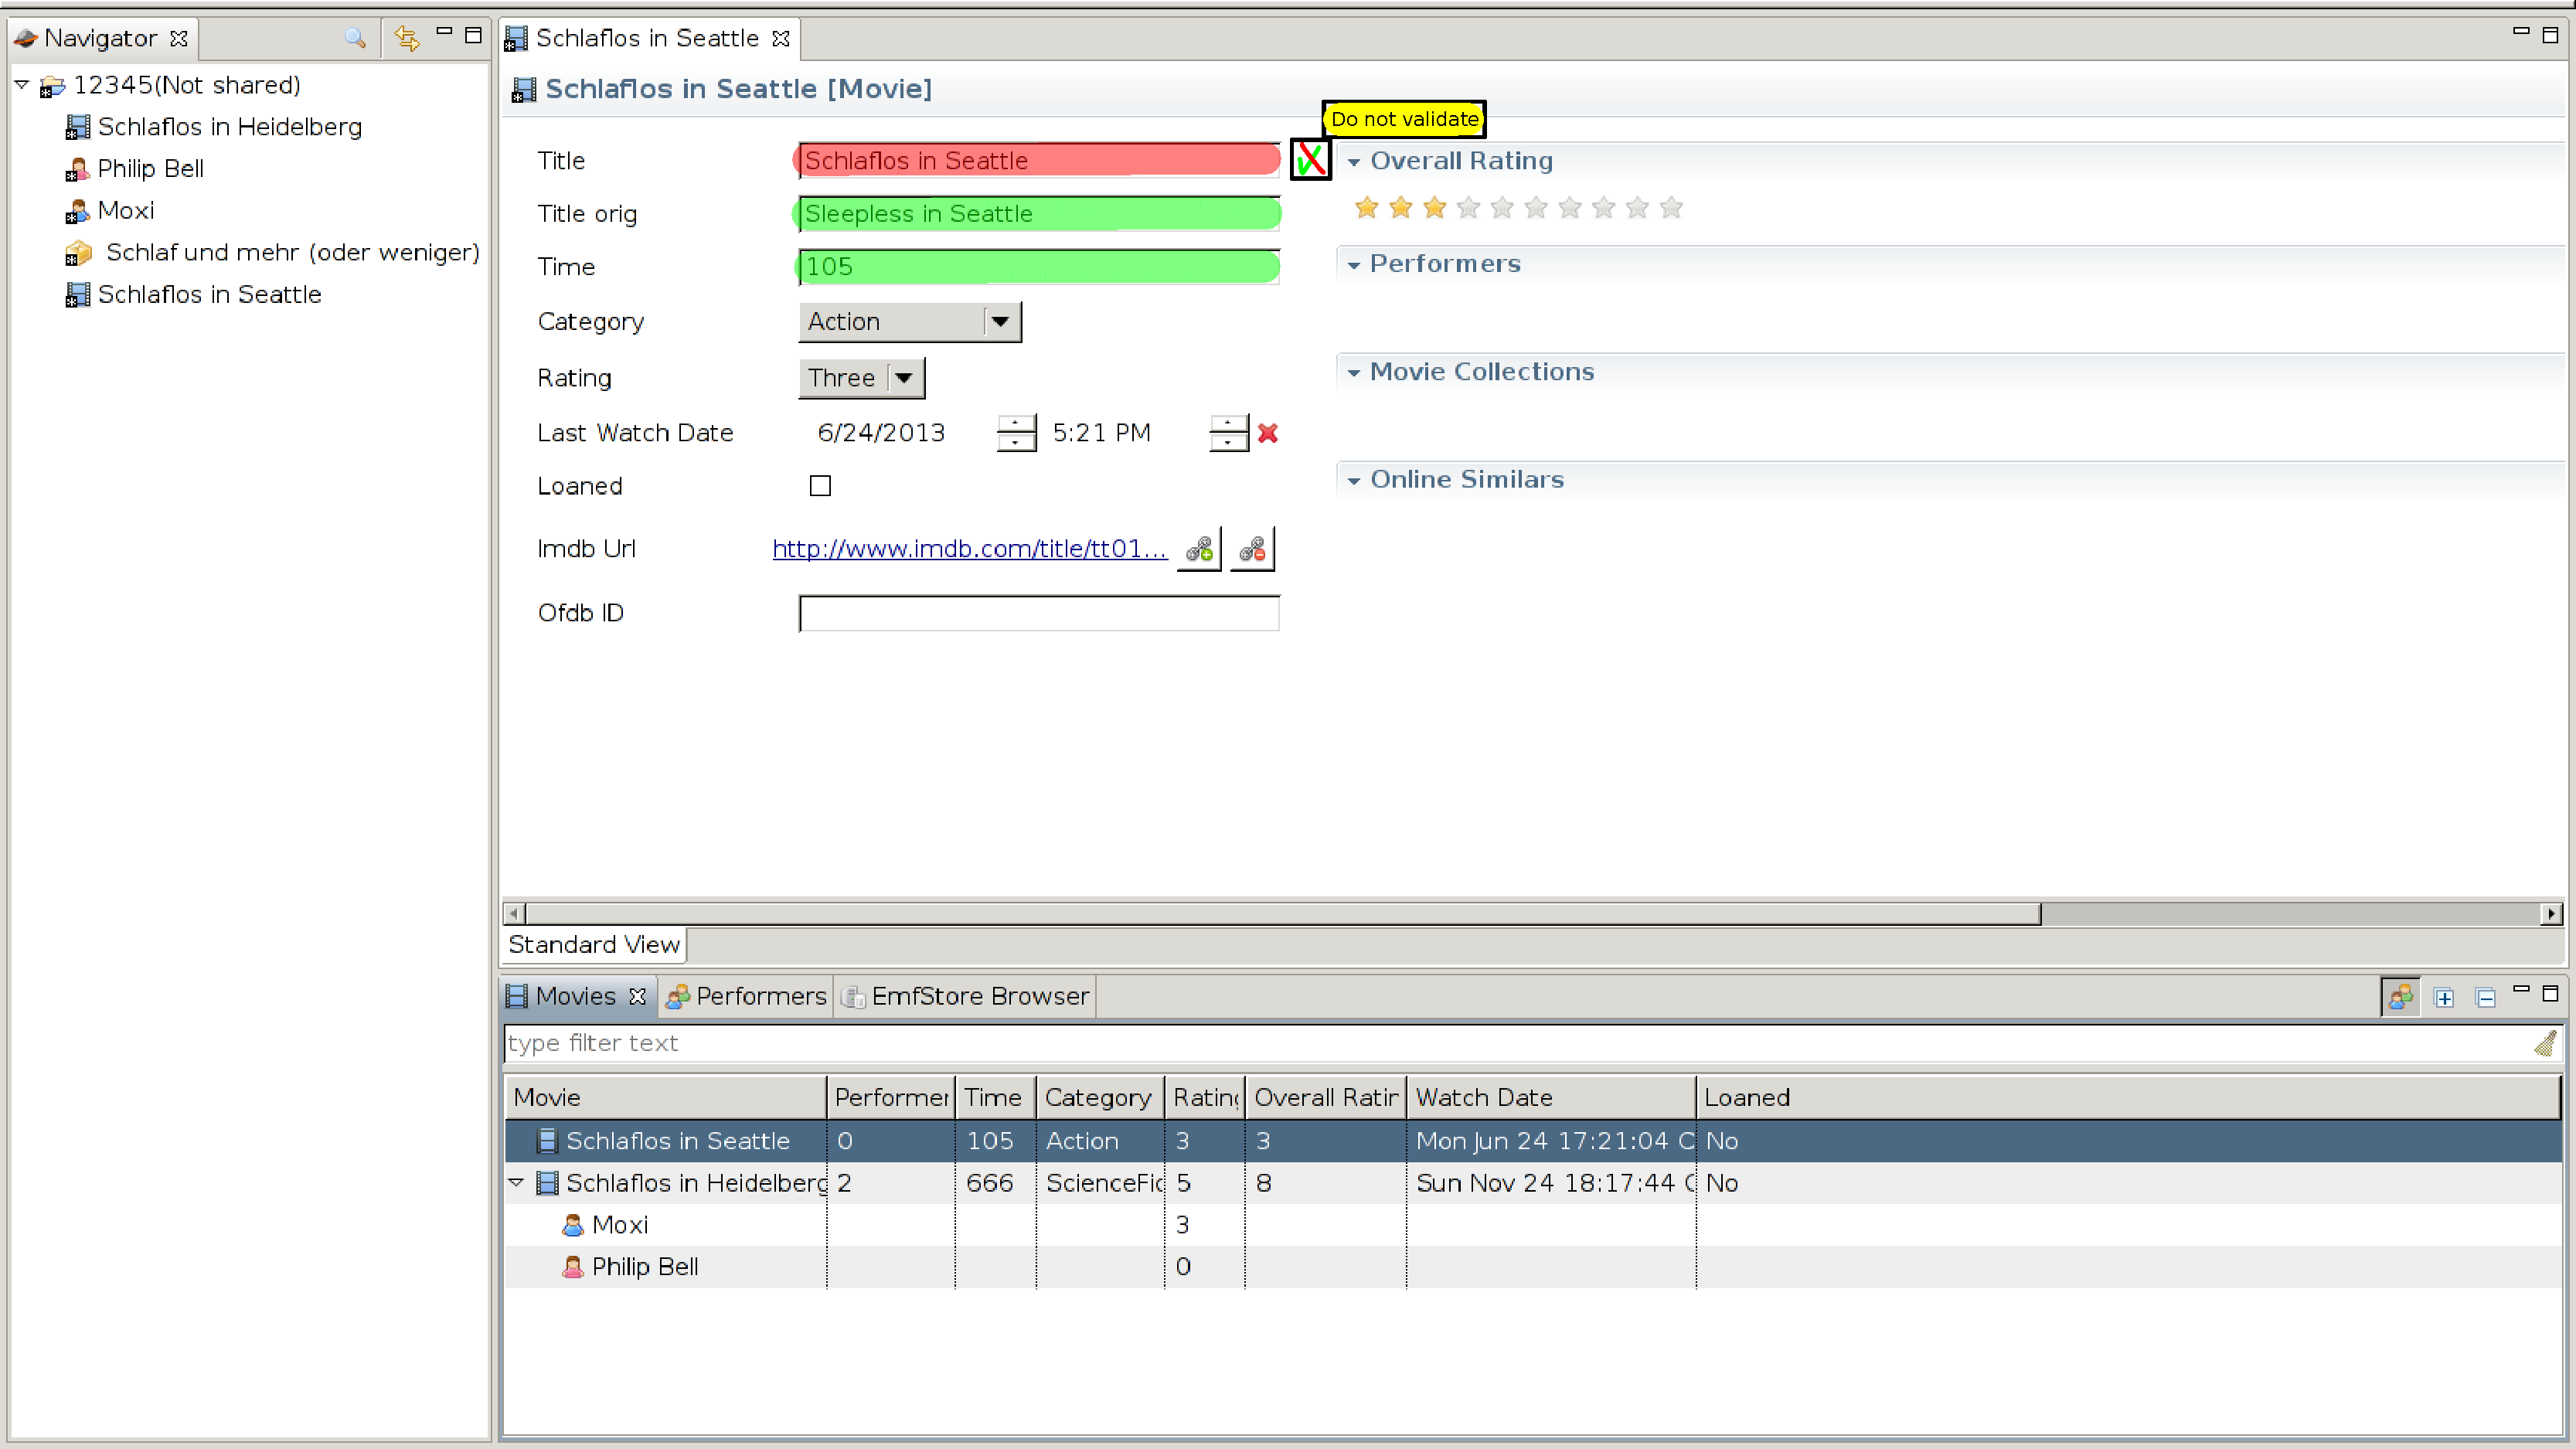
\includegraphics[width=\linewidth]{moviemanager_all_annotaded}
			%\caption{Tuchulcha with a (very) simple workflow, picture taken from \cite{tuchulcha-website}}
		\end{figure}
	\end{frame}
	%}}}

	%{{{
	\section{}
	\begin{frame}
		\center{\Huge ENDE}
	\end{frame}
	%}}}

\end{document}
%}}}
